\documentclass[a4paper,11pt]{article}

\usepackage[french]{babel}
\usepackage[T1]{fontenc}
\usepackage[utf8]{inputenc}
\usepackage{graphicx}
\usepackage{hyperref}
%\usepackage{fullpage}

\begin{document}

\title{\textbf{Compte rendu du TP \no 2}\\Code d'Huffman et code prédictif}
\author{Thibaut Castanié\\\textit{M2 IMAGINA}}
\date{\today}

\maketitle
\thispagestyle{empty}

\newpage 

\section{Image choisie}

\begin{center}
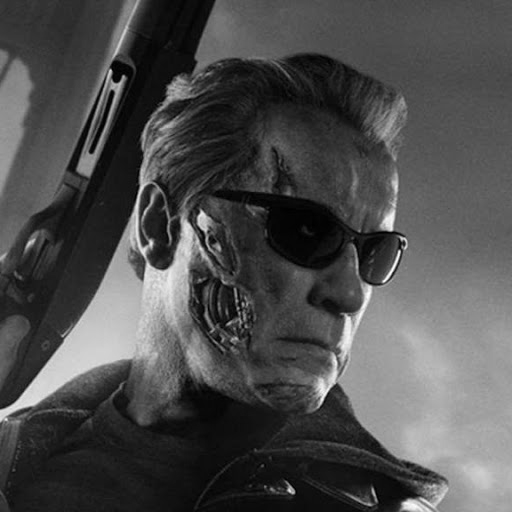
\includegraphics[scale=0.5]{./terminator.png}\\
\textit{L'image .pgm utilisée pour le TP}
\end{center}


\section{Dans l'espace des pixels}

Afin d'avoir une idée des probabilités d'apparition de chaque niveau de gris, on trace l'histogramme de l'image. Pour l'afficher, l'utilitaire \texttt{gnuplot} est utilisé.

\begin{center}
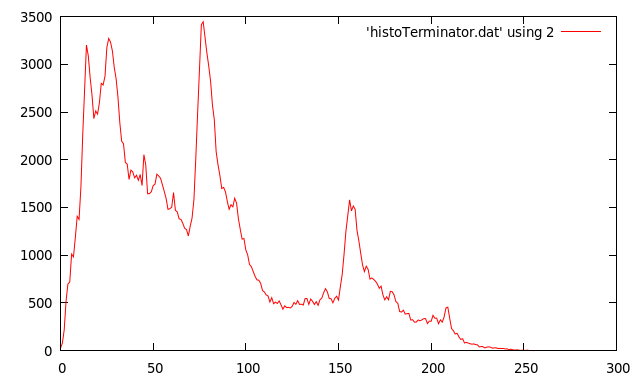
\includegraphics[scale=0.5]{./histoTerminatorPGM_GNU.png}\\
\textit{Histogramme de l'image terminator.pgm}
\end{center}

L'algorithme d'Huffman utilisé pour ce TP provient du site communautaire RosetaCode.org (\href{http://rosettacode.org/wiki/Huffman_coding#C.2B.2B}{{http://rosettacode.org/wiki/Huffman\_coding\#C++}}).

L'algorithme utilise une \textit{map}, il suffit alors de la remplir avec les pixels de notre image.

\begin{verbatim}
for (int i = 0; i < nW; i++){
    for (int j = 0; j < nH; j++){
        frequencies[ImgIn[i*nW+j]]++;
    }
}
\end{verbatim}

On créé un fichier compressé avec l'algorithme de Huffman, chaque octet étant codé sur 8 bits, on concatène les représentation de chaque symboles. On obtient ainsi un fichier binaire compressé.

\vspace{0,5cm}

\begin{itemize}
\item Taille \textit{terminator.pgm} : 262 198 octets.
\item Taille \textit{terminatorComp.comp} : 187 011 octets.
\end{itemize}

\vspace{0,2cm}

\textbf{Taux de compression} : $\tau = \frac{262 198}{187 011} = 1.402045 \approx 1.4$


\section{Dans l'espace de prédilection}

En utilisant une méthode de prédiction des voisins, on obtient la carte des différences suivante.

\begin{center}
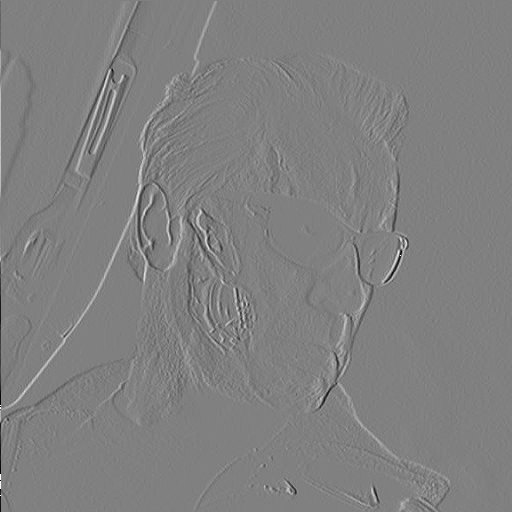
\includegraphics[scale=0.5]{./terminatordiff.png}\\
\textit{Carte des différences de terminator.pgm}
\end{center}

Ensuite, on passe de nouveau l'image dans l'algorithme d'Huffman, et on obtient les chiffres suivants :

\vspace{0,5cm}

\begin{itemize}
\item Taille \textit{terminatorDiff.pgm} : 262 159 octets.
\item Taille \textit{terminatorDiffComp.comp} : 62 650 octets.
\end{itemize}

\vspace{0,2cm}

\textbf{Taux de compression} : $\tau = \frac{262 159}{62 650} = 4.184501 \approx 4.2$



\section{Comparaison et conclusion}

En utilisant l'espace des pixels, on obtient un taux de \textbf{1,4}. En utilisant l'espace de prédilection, on obtient un bon taux de \textbf{4,2}. Ainsi ce dernier est bien plus efficace, en raison de la probabilité d'apparition d'un petit nombre de pixels bien plus élevée.

Afin d'obtenir un meilleur taux de compression, nous pouvons utiliser l'algorithme de LZW qui utilise un dictionnaire. Il est même possible d'utiliser Huffman et LZW l'un après l'autre.

En septembre dernier, une équipe travaillant pour Google a sorti l'algorithme Brotli qui est basé sur une version modifiée de LZ77, le codage de Huffman et un modelage du contexte de second ordre. Cet algorithme est 20\% plus performant dans son taux de compression que les algorithmes de compression utilisés jusqu'ici.


\end{document}